\documentclass[12pt,onecolumn,draftclsnofoot]{IEEEtran}
\usepackage[a4paper,margin=1in]{geometry}
\usepackage{times,graphicx,amsmath,booktabs,cite,url}
\usepackage[ruled,linesnumbered]{algorithm2e}
% Added beyond the given preamble: diagrams and plots are drawn in LaTeX (no screenshots).
\usepackage{tikz,pgfplots,tabularx,array}
\usetikzlibrary{arrows.meta,positioning,fit,calc}
\pgfplotsset{compat=1.18, every node near coord/.append style={/pgf/number format/fixed, /pgf/number format/fixed zerofill, /pgf/number format/precision=2}}
\newcolumntype{Y}{>{\raggedright\arraybackslash}X}
\setlength{\emergencystretch}{3em} % lets justified lines absorb long \texttt tokens

\begin{document}

\title{Ontology-Typed GraphRAG with an AI-Assisted DevOps Pipeline for Question Answering over Company Email}

% TODO(team): replace names and roll numbers; keep only YOUR instructor's name (Naveen Singh OR Kiran Khatter) and your group number.
\author{Group XX: Name1 (Roll No.), Name2 (Roll No.), Name3 (Roll No.), Naveen Singh/Kiran Khatter\\
School of Engineering \& Technology, BML Munjal University}

\maketitle

\begin{abstract}
Small companies keep most of their decisions in email, and the person who asks ``why was this decided'' rarely knows which thread holds the answer. Retrieval-augmented generation (RAG) over text chunks finds passages that share words with the question, but it misses answers that are linked to the question only through a person, a decision or a reason. We present Lore, a question-answering system built with a real client, EZO Books, that extracts an ontology-typed knowledge graph from 11,584 email threads and answers by expanding that graph from vector seeds, reranking with a cross-encoder and generating a cited answer. Lore is delivered through an AI-assisted DevOps workflow: a GitLab pipeline with a coverage-gated test stage fed by a generate-run-keep test generator, warn-only security scans, GitOps promotion, and a Terraform stack that deploys the full system to AWS in one command. On a frozen golden set of 55 relationship questions with Cypher-derived ground truth, Lore reaches node recall@10 of 0.40 against 0.14 for node-level vector RAG (paired difference +0.26, 95\% CI [+0.13, +0.40]). On 60 single-email lookups it loses (hit@10 0.40 against 0.75). A 2$\times$2 ablation shows why: LLM query analysis adds +0.32 on person-and-topic questions but costs $-0.23$ on lookups, and the reranker recovers +0.27. The AI test generator raised three modules to full line coverage and rejected a fourth. The results suggest that typed graphs are worth their latency only for relationship questions, so a router should send lookups to plain retrieval.
\end{abstract}

\begin{IEEEkeywords}
Continuous delivery, GitOps, knowledge graphs, large language models, retrieval-augmented generation, test generation
\end{IEEEkeywords}

% TODO(team): paste the real Overleaf project link.
\noindent\textbf{Overleaf Project Link:} \url{https://www.overleaf.com/project/...}\\
\textbf{Code Repository:} \url{https://github.com/ninadw25/AI_devops_loremind}

\section{Introduction}

Retrieval-augmented generation lets a language model answer from documents it was never trained on: a retriever selects passages and the model writes an answer grounded in them \cite{lewis2020rag}. It has become the default way companies put an assistant on top of their own records, because it needs no fine-tuning and its answers can cite their sources \cite{gao2023ragsurvey}. For a small or medium business the most valuable record is usually email. Approvals, assignments and the reasons behind them are written there once and are hard to find again, especially after the person who wrote them has left.

The need is practical rather than academic. When an employee leaves, a handover note covers a fraction of what they decided; when a new hire joins, they learn the history of a client or a product by asking the people who were there. In a firm of fifty people, a few senior staff answer these questions all day, and the answers they give are already written down, scattered across thousands of threads. An assistant that could answer them with citations would save senior time and keep knowledge when people leave. Building one is also a DevOps problem: an LLM system can change its behaviour without any change to its code, when a dependency fails to install, a model endpoint slows down or a timeout fires, so it has to be tested, measured and deployed with the same discipline as any other service.

The questions people ask about this history are rarely lookups of one message. A manager asks what tasks were assigned to a colleague, why a vendor was rejected, or what a director decided about pricing. The text that answers such a question often does not contain the words of the question. In our client's mail, only 4\% of the task descriptions assigned to a person contain any part of that person's name; the link between the two exists only in the structure of the conversation. A chunk retriever ranks by textual similarity, so it cannot see that link. Engineers who build these assistants face a second difficulty: retrieval pipelines combine several models and thresholds, and a component that silently falls back to a weaker mode can lower answer quality without failing any test \cite{barnett2024failure}.

Graph-based RAG addresses the first difficulty by retrieving over entities and relations rather than chunks \cite{edge2024graphrag,peng2024graphragsurvey}. Systematic comparisons, however, find that graphs help on multi-hop questions and hurt on single-hop detail questions \cite{han2025ragvsgraphrag,xiang2025graphragbench}, and most published results use public benchmarks rather than a company's private mail. Work on ontology-guided graph construction reports gains from a fixed schema \cite{dacruz2025ontology,wang2026omdgraphrag}, but does not measure which query-time components cause the gain, or how such a system is tested and shipped. Coverage-guided test generation with LLMs has been shown in industry \cite{alshahwan2024testgen}, yet it is rarely connected to the pipeline that delivers an LLM system itself.

We therefore ask two research questions. \textbf{RQ1:} Does retrieval over an ontology-typed email graph improve node recall@10 over vector RAG on relationship questions, and what does it cost on single-email lookups and in latency? \textbf{RQ2:} Which query-time component, LLM query analysis or cross-encoder reranking, causes those gains and losses?

The paper makes four contributions:
\begin{itemize}
\item An end-to-end system, built with a real client, that turns email into a typed knowledge graph and answers with cited sources through graph expansion, hybrid ranking and a cross-encoder.
\item A judge-free evaluation on a frozen golden set of 115 questions, where ground truth comes from Cypher traversals and source threads rather than from an LLM grader, with paired bootstrap intervals.
\item A 2$\times$2 ablation that separates the effect of LLM query analysis from the reranker and exposes an interaction between them.
\item A DevOps workflow for an LLM system: a coverage-gated CI stage fed by an LLM test generator that keeps a test only if it passes and raises coverage, GitOps promotion, and a one-command infrastructure-as-code deployment that stores no access keys.
\end{itemize}

Section II reviews related work, Section III defines the problem, Section IV describes the method, Section V the experimental setup, Section VI the results, Section VII discusses them, and Section VIII concludes.

\section{Related Work}

\subsection{Retrieval-augmented generation and its failure modes}
Lewis et al.\ combined a dense retriever with a sequence-to-sequence generator and showed that retrieval improves factual question answering \cite{lewis2020rag}. Gao et al.\ survey the many variants that followed, from simple retrieve-then-read pipelines to modular systems with query rewriting and reranking \cite{gao2023ragsurvey}. Barnett et al.\ studied three deployed RAG systems and listed seven points where they fail, including missed top-ranked documents and relevant text that never reaches the context \cite{barnett2024failure}; we use their list to classify our own failures. Self-RAG and CRAG add a step that judges retrieval quality and reacts to it, by reflection tokens or by a corrective retrieval action \cite{asai2023selfrag,yan2024crag}. These methods improve retrieval over text but still rank passages by content, not by the relations between the people and decisions they mention. They also add model calls to every request, and Barnett et al.\ note that each added stage is one more place where a system can degrade quietly. Our engine borrows only the cheapest part of this idea: a confidence label computed from retrieval scores and shown to the user, without corrective re-retrieval. A conversational assistant also needs memory across turns. MemGPT treats the model's context as a small main memory and pages older conversation in and out of external storage, much like an operating system \cite{packer2023memgpt}. Our requirement is narrower, follow-up questions in one thread, so Lore keeps the ten most recent turns of a thread in PostgreSQL, checks on every read that the thread belongs to the user, and adds them to the synthesis prompt; paging and summarisation are not needed at that length.

\subsection{Graph-based RAG}
Edge et al.\ build an entity graph with an LLM, summarise its communities and show that the summaries answer corpus-wide ``sensemaking'' questions better than chunk retrieval \cite{edge2024graphrag}. HippoRAG runs personalised PageRank from the entities in a question and improves multi-hop retrieval at lower cost than iterative retrieval \cite{gutierrez2024hipporag}. Peng et al.\ organise the field into graph indexing, graph-guided retrieval and graph-enhanced generation \cite{peng2024graphragsurvey}, and Pan et al.\ describe the wider space of KG-enhanced LLMs, LLM-augmented KGs and systems where the two reason together \cite{pan2024unifying}; Lore sits in the second group at build time and the first at query time. Two recent evaluations temper the enthusiasm: Han et al.\ find that RAG is better on single-hop detail and GraphRAG on multi-hop reasoning \cite{han2025ragvsgraphrag}, and GraphRAG-Bench reports that graphs often underperform vanilla RAG unless the task needs relational reasoning \cite{xiang2025graphragbench}. Our two test sets were designed to check exactly this split on private data. A limitation shared by these studies is that their corpora are public and their questions are written by annotators who know the documents; organisational mail is noisier, full of forwarded chains and signatures, and the people asking do not know which thread holds the answer. Community summaries also have a cost that matters to a small company: they must be rebuilt as mail arrives, which is why Lore detects corpus-wide questions but does not yet serve them.

\subsection{Ontology-guided graph construction}
Free-form triple extraction produces many near-duplicate relation names. da Cruz et al.\ compare ontology-learning approaches and measure their effect on downstream RAG \cite{dacruz2025ontology}, and OMD-GraphRAG guides extraction with an ontology before clustering and fusing graph and text channels \cite{wang2026omdgraphrag}. Lore follows the same principle with a smaller, fixed schema of seven node types, chosen with the client, and a deterministic validator before any write.

\subsection{Ranking and indexing}
BM25 remains a strong lexical baseline \cite{robertson2009bm25}, and cross-encoders trained on large passage-ranking data rerank candidates by reading the question and the passage together \cite{nogueira2019rerank}. FAISS provides exact and approximate vector search and is the index behind our baselines \cite{johnson2017faiss}. Semantic code search, benchmarked by CodeSearchNet \cite{husain2019codesearchnet}, motivates the code-question mode of our system. The usual design pairs a cheap first stage that favours recall with an expensive second stage that favours precision. We keep that design but add a graph stage between them, so the cross-encoder sees candidates reached through relations as well as through similarity. Cross-encoders score text only and ignore graph provenance, which we found to matter when the right answer shares few words with the question.

\subsection{Evaluation and AI in the delivery pipeline}
RAGAS scores faithfulness and relevance with an LLM judge and needs no ground truth \cite{es2023ragas}; we chose the opposite design, ground truth from the graph, so that no model grades its own output. On the delivery side, continuous delivery argues for small, automated, reversible releases \cite{humble2010cd}, and Meta's TestGen-LLM showed that LLM-written tests can be filtered automatically so that only passing tests that add coverage are kept \cite{alshahwan2024testgen}. We reuse that filter inside our CI gate. Its value for a small team is that it turns an unreliable generator into a safe one: a test that fails or adds nothing never reaches the repository, so the gate cannot be weakened by generated code. Line coverage, however, says nothing about whether a test would catch a fault, a limitation that applies to our use as well.

Table~\ref{tab:related} compares the eight works closest to ours. It can be observed that none of them combines a private organisational corpus, a component-level ablation and a delivery pipeline. The gap we address is therefore practical: whether a typed graph helps on one company's real mail, which component is responsible, and how such a system can be tested and shipped by a small team.

\begin{table}[t]
\centering
\caption{Comparison of closely related work}
\label{tab:related}
\footnotesize
\begin{tabularx}{\textwidth}{@{}p{2.3cm}YYYY@{}}
\toprule
Work & Problem and method & Data and metric & Key result & Limitation and relevance to Lore \\
\midrule
Lewis et al.\ \cite{lewis2020rag} & Dense retrieval + generator & Open-domain QA; exact match & Retrieval improves factual QA & Text chunks only; our baseline family \\
Edge et al.\ \cite{edge2024graphrag} & LLM entity graph + community summaries & Podcast and news corpora; LLM-judged win rate & Better on corpus-wide questions & No typed schema; we use its local-search idea \\
Gutiérrez et al.\ \cite{gutierrez2024hipporag} & KG + personalised PageRank & Multi-hop QA benchmarks; recall & Better multi-hop retrieval, cheaper than iteration & Public data; candidate fix for our hub failures \\
Han et al.\ \cite{han2025ragvsgraphrag} & Systematic RAG vs.\ GraphRAG study & Several QA benchmarks & Graph helps multi-hop, hurts single-hop & Motivates our two test sets \\
Xiang et al.\ \cite{xiang2025graphragbench} & Benchmark of graph RAG & GraphRAG-Bench tasks & Graphs often lose to vanilla RAG & Motivates per-family reporting \\
da Cruz et al.\ \cite{dacruz2025ontology} & Ontology learning for KG construction & RAG QA tasks & Schema choice changes RAG quality & Closest construction approach \\
Barnett et al.\ \cite{barnett2024failure} & Case studies of deployed RAG & Three systems; qualitative & Seven failure points & Our failure taxonomy \\
Alshahwan et al.\ \cite{alshahwan2024testgen} & LLM test generation with filters & Meta codebases; coverage, acceptance & Filtered tests accepted by engineers & Algorithm behind our CI test loop \\
\bottomrule
\end{tabularx}
\end{table}

\section{Background and Problem Formulation}

A \emph{knowledge graph} $G=(V,E)$ stores nodes $v\in V$ with a label $\ell(v)$ and typed edges $(u,r,v)\in E$ with relation $r$. Lore's ontology has three \emph{spine} labels shared across threads (Person, Organization, Topic) and four \emph{content} labels extracted per thread (Decision, Task, Fact, Event). Relations include ASSIGNED\_TO (Task to Person), DECIDED (Person to Decision), BECAUSE (Decision to Fact) and REGARDING (content to Topic). Every content node carries a text description, a 2048-dimensional embedding, its source thread id and a set of access scopes. A \emph{bi-encoder} embeds question and text separately so that candidates can be found by nearest-neighbour search; a \emph{cross-encoder} reads both together and gives a sharper but slower score \cite{nogueira2019rerank}. Because the bi-encoder can be precomputed for every node and the cross-encoder cannot, retrieval systems use the first to shortlist and the second to reorder. An \emph{access scope} is an identifier attached to a node during ingestion, such as a mailbox or a Slack channel; a user may see a node only if one of the user's scopes matches. \emph{GitOps} is a deployment practice in which the desired state of a cluster is stored in a Git repository and an agent such as Argo CD continuously makes the cluster match it, so every deployment and every rollback is a commit \cite{argocd2026docs}. Table~\ref{tab:notation} lists the notation used in the rest of the paper.

\begin{table}[t]
\centering
\caption{Notation}
\label{tab:notation}
\footnotesize
\begin{tabular}{@{}ll@{}}
\toprule
Symbol & Meaning \\
\midrule
$q$, $S_q$ & question and the access scopes of the user who asks it \\
$G=(V,E)$, $\ell(v)$ & knowledge graph and the label of node $v$ \\
$\iota$ & intent of $q$ (e.g.\ TASK\_LOOKUP, REASONING) from query analysis \\
$w_r$, $h_d$ & weight of relation $r$; penalty for hop depth $d$ \\
$\pi_{\iota,r}$, $\lambda_{\iota,\ell}$ & intent prior for relation $r$; intent boost for label $\ell$ \\
$B$, $D$ & beam width and maximum expansion depth \\
$\alpha$, $\beta$ & weights of graph score and BM25 score in the hybrid score \\
$w_1$, $w_2$ & weights of rerank score and hybrid score in the final score \\
$\mathcal{G}_q$, $R_k(q)$ & ground-truth node set of $q$; top-$k$ retrieved list \\
\bottomrule
\end{tabular}
\end{table}

\textbf{Problem.} Given a question $q$, the scopes $S_q$ and the graph $G$, return a ranked list $R_k(q)$ of at most $k=10$ content nodes, and an answer that cites them, such that $R_k(q)$ contains as many nodes of $\mathcal{G}_q$ as possible. \textbf{Assumptions:} the graph has already been built by ingestion and is read-only at query time; a node with no scopes is invisible to everyone (fail-closed). \textbf{Constraints:} answers must be streamed within interactive time on a CPU-only server; no customer data may leave the company's cloud account except to the LLM endpoint inside it. \textbf{Out of scope:} corpus-wide summary questions (``what were the main themes this quarter''), which the engine detects but does not yet serve, and the quality of the generated answer text, which we do not score.

\section{Proposed Methodology}

\subsection{System architecture}
Fig.~\ref{fig:arch} shows the components and how they connect. Ingestion runs offline per source. For Gmail it filters noise with header and sender signals, resolves the same person across addresses and domains, groups messages by thread, asks an LLM to extract typed nodes and edges from each thread, and passes the output through a deterministic validator before writing to Neo4j. Thread-level extraction reduces the number of LLM calls by an order of magnitude compared with one call per message. The query engine is a FastAPI service that reads the graph, keeps conversation memory in PostgreSQL, and calls Claude 3.5 Sonnet on AWS Bedrock for query analysis and answer synthesis. A code-question mode answers questions about the client's GitLab history (1,840 commits, 160 files) through structured queries and vector search over commits and symbols. Caddy terminates TLS, enforces a password, and injects the engine's internal secret server-side so that it never reaches the browser.

\begin{figure}[t]
\centering
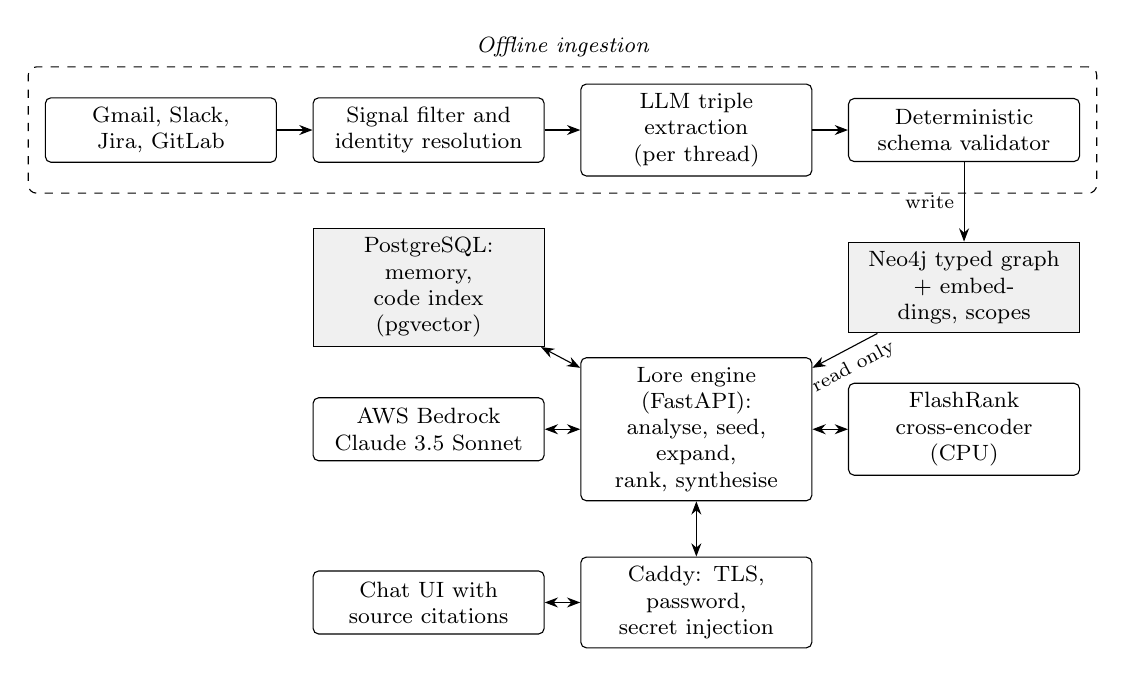
\begin{tikzpicture}[
  font=\linespread{1}\footnotesize, >=Stealth, node distance=4mm and 7mm,
  box/.style={draw, rounded corners=2pt, align=center, minimum height=8mm, text width=27mm, fill=white},
  store/.style={draw, align=center, minimum height=8mm, text width=27mm, fill=black!6},
  grp/.style={draw, dashed, rounded corners=3pt, inner sep=6pt}]
\node[box] at (0,0) (src) {Gmail, Slack,\\Jira, GitLab};
\node[box] at (34mm,0) (filt) {Signal filter and\\identity resolution};
\node[box] at (68mm,0) (ext) {LLM triple extraction\\(per thread)};
\node[box] at (102mm,0) (val) {Deterministic\\schema validator};
\node[store] at (102mm,-20mm) (neo) {Neo4j typed graph\\+ embeddings, scopes};
\node[store] at (34mm,-20mm) (pg) {PostgreSQL: memory,\\code index (pgvector)};
\node[box] at (68mm,-38mm) (eng) {Lore engine (FastAPI):\\analyse, seed, expand,\\rank, synthesise};
\node[box] at (102mm,-38mm) (rr) {FlashRank\\cross-encoder (CPU)};
\node[box] at (34mm,-38mm) (llm) {AWS Bedrock\\Claude 3.5 Sonnet};
\node[box] at (68mm,-60mm) (cad) {Caddy: TLS, password,\\secret injection};
\node[box] at (34mm,-60mm) (ui) {Chat UI with\\source citations};
\draw[->] (src) -- (filt); \draw[->] (filt) -- (ext); \draw[->] (ext) -- (val);
\draw[->] (val) -- node[left, font=\scriptsize]{write} (neo);
\draw[->] (neo) -- node[sloped, below, font=\scriptsize]{read only} (eng);
\draw[<->] (pg) -- (eng);
\draw[<->] (llm) -- (eng); \draw[<->] (rr) -- (eng);
\draw[<->] (eng) -- (cad); \draw[<->] (cad) -- (ui);
\node[grp, fit=(src)(filt)(ext)(val), label={[font=\footnotesize\itshape]above:Offline ingestion}] {};
\end{tikzpicture}
\caption{Architecture of Lore. Ingestion writes a typed graph once; the engine reads it at query time and calls an LLM only for query analysis and answer synthesis.}
\label{fig:arch}
\end{figure}

\subsection{Query workflow}
Fig.~\ref{fig:flow} shows the step-by-step path from a question to an answer, and Algorithm~\ref{alg:query} gives it in pseudocode. Embedding and query analysis run concurrently. The analysis prompt asks the LLM for a JSON object with an intent from a closed list, the people and topics named, and a time range; the output is parsed and validated, and any error, schema violation or timeout falls back to a deterministic keyword classifier. We designed the prompt as a closed-vocabulary classification rather than a free rewrite because a closed list can be validated and has a deterministic fallback, which keeps the engine answering when the LLM is slow.

\begin{figure}[t]
\centering
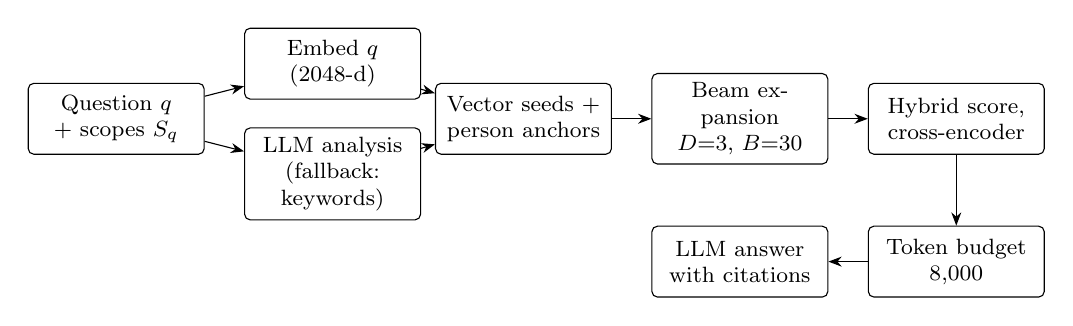
\begin{tikzpicture}[font=\linespread{1}\footnotesize, >=Stealth, node distance=5mm,
  st/.style={draw, rounded corners=2pt, align=center, minimum height=9mm, text width=20mm, fill=white}]
\node[st] (q) {Question $q$\\+ scopes $S_q$};
\node[st, right=of q, yshift=7mm] (emb) {Embed $q$\\(2048-d)};
\node[st, right=of q, yshift=-7mm] (an) {LLM analysis\\(fallback: keywords)};
\node[st, right=13mm of $(emb)!0.5!(an)$] (seed) {Vector seeds +\\person anchors};
\node[st, right=of seed] (exp) {Beam expansion\\$D{=}3$, $B{=}30$};
\node[st, right=of exp] (rank) {Hybrid score,\\cross-encoder};
\node[st, below=9mm of rank] (cut) {Token budget\\8,000};
\node[st, left=of cut] (syn) {LLM answer\\with citations};
\draw[->] (q) -- (emb); \draw[->] (q) -- (an);
\draw[->] (emb) -- (seed); \draw[->] (an) -- (seed);
\draw[->] (seed) -- (exp); \draw[->] (exp) -- (rank); \draw[->] (rank) -- (cut); \draw[->] (cut) -- (syn);
\end{tikzpicture}
\caption{Query workflow from question to cited answer. The scope gate is applied inside every graph query, so out-of-scope nodes never enter the candidate set.}
\label{fig:flow}
\end{figure}

\begin{algorithm}[t]
\caption{Lore query pipeline}
\label{alg:query}
\KwIn{question $q$, scopes $S_q$, graph $G$, parameters $B, D, \tau, T$}
\KwOut{answer $a$ and cited nodes $C$}
In parallel: $e \leftarrow \mathrm{Embed}(q)$; $A \leftarrow \mathrm{Analyse}(q)$ with deadline $\tau$\;
\If{$A$ timed out or failed validation}{$A \leftarrow \mathrm{KeywordAnalysis}(q)$}
$F \leftarrow \mathrm{ANN}(e, 30) \cup \mathrm{PersonAnchors}(A)$, keeping only nodes visible under $S_q$\;
$P \leftarrow F$\;
\For{$d \leftarrow 1$ \KwTo $D$}{
  $N \leftarrow$ neighbours of $F$ along relations allowed for each label, under the scope gate\;
  score each $v\in N$ by Eq.~(\ref{eq:frontier}); keep the best path per node; apply the convergence bonus\;
  $F \leftarrow$ top $B$ of $N$; $P \leftarrow P \cup F$\;
}
compute $h(v)$ by Eq.~(\ref{eq:hybrid}) and $f(v)$ by Eq.~(\ref{eq:final}) for $v\in P$; sort by $f$\;
$C \leftarrow$ longest prefix of the sorted list within $T$ tokens\;
$a \leftarrow \mathrm{Synthesise}(q, C)$, streamed with source citations\;
\Return{$a, C$}
\end{algorithm}

\subsection{Scoring}
During expansion a node $v$ reached from parent $u$ over relation $r$ at depth $d$ gets
\begin{equation}
s(v) = s(u)\cdot w_r \cdot h_d \cdot \pi_{\iota,r} \cdot \lambda_{\iota,\ell(v)},
\label{eq:frontier}
\end{equation}
where $w_r\in[0.3,1.0]$ is a relation weight (BECAUSE $=1.0$, ASSIGNED\_TO $=0.8$, COMMUNICATES\_WITH $=0.3$), $h_d\in\{1.0, 0.8, 0.6\}$ the hop penalty, $\pi_{\iota,r}$ an intent prior (for example $1.8$ for BECAUSE under REASONING) and $\lambda_{\iota,\ell}$ an intent label boost. When several paths reach $v$, the best score is kept and multiplied by $1+\gamma(p_v-1)$, where $p_v$ is the number of paths and $\gamma=0.1$. Candidates are then ranked by a hybrid score
\begin{equation}
h(v) = \alpha\,\hat{g}(v) + \beta\,\hat{b}(v),
\label{eq:hybrid}
\end{equation}
where $\hat{g}$ and $\hat{b}$ are the min-max normalised graph and BM25 scores \cite{robertson2009bm25} and $\alpha=0.6$, $\beta=0.4$; if the BM25 library is absent, $h=\hat{g}$. Finally,
\begin{equation}
f(v) = w_1\,\hat{c}(v) + w_2\,h(v),
\label{eq:final}
\end{equation}
where $\hat{c}$ is the normalised cross-encoder score and $w_1=0.7$, $w_2=0.3$. If the reranker fails, the engine logs the degradation and ranks by $h$ alone.

\subsection{Design choices}
\emph{Typed graph instead of chunks}: the client's questions are about people, decisions and reasons, which are relations; a fixed schema of seven labels keeps relation names consistent, unlike free-form extraction \cite{dacruz2025ontology}. \emph{Beam expansion instead of personalised PageRank}: a beam with intent priors is cheap to run per request in Cypher and easy to explain; PageRank \cite{gutierrez2024hipporag} is a candidate for the hub failure we report. \emph{FlashRank MiniLM cross-encoder}: it runs on CPU in the same container, so no text leaves the server for reranking and no extra service is paid for. \emph{Claude 3.5 Sonnet on Bedrock}: the model is reached through the instance's IAM role inside the company's AWS account, so there is no separate vendor key to store or rotate. \emph{Same embedding model for every system}: \texttt{nemotron-3-embed-1b} is used by Lore and both baselines, so differences come from structure, not from embeddings. \emph{Beam width 30, depth 3}: weights beyond three hops are below $0.6^3$ of the seed score and add latency without useful candidates.

\subsection{DevOps workflow}
Fig.~\ref{fig:cicd} shows how a change reaches users. Every merge request runs lint, a unit-test stage and SAST and secret scans in GitLab CI. The unit-test stage is the hard gate: it fails the pipeline below 65\% line coverage. Lint and the security scans are deliberately warn-only, so findings are visible on the merge request without blocking a small team; turning them into gates is a separate, deliberate decision. Tests in the gated stage include tests written by an LLM through a generate-run-keep loop: for a target module the generator is given the source and its uncovered lines, writes a test file, runs it, and keeps it only if every test passes and module coverage rises; a failing file is sent back with the error, at most three times. This is the filter used by TestGen-LLM \cite{alshahwan2024testgen}; we reimplemented it because Qodo Cover, the open-source tool that packaged it, is archived. The build stage pushes an image tagged with the commit hash to ECR. Deployment is GitOps: CI changes one image tag in a Git repository and ArgoCD makes the Kubernetes cluster match it, first in staging and, after a manual promote, in production, so rollback is a revert of one commit \cite{humble2010cd}. The retrieval benchmark is a manual job that runs only on the default branch, because it needs database and model credentials that merge-request code must never receive.

For the evaluated system we also wrote a self-contained Terraform stack. A script packs the graph, a database dump, the engine source and the built UI into a private S3 bucket, writes secrets to SSM Parameter Store as encrypted strings, and produces a saved plan; a second command applies exactly that plan. Terraform creates 17 resources: an EC2 instance whose boot script installs Docker and starts four containers (Caddy, engine, Neo4j, PostgreSQL), an IAM role that grants only bundle read, parameter read and Bedrock invoke, a security group with ports 80 and 443 open and no SSH, and a DNS record. Administration goes through AWS Systems Manager. We reviewed the stack against the AWS Well-Architected Framework \cite{aws2024wellarchitected}. For \emph{security}, the instance holds no access keys and reaches Bedrock, S3 and SSM through a least-privilege role, secrets are encrypted parameters, and there is no SSH port. For \emph{operational excellence}, the environment is code with a reviewed plan, so it can be rebuilt rather than repaired. For \emph{cost optimisation}, one instance is created only when needed and destroyed with one command. The deliberate trade-off is \emph{reliability}: a single instance in one zone has no failover, which is acceptable for a demonstration and not for production. We chose one instance over the production Kubernetes cluster because the demo runs for days, not months, and should not share failure or cost with live services.

\begin{figure}[t]
\centering
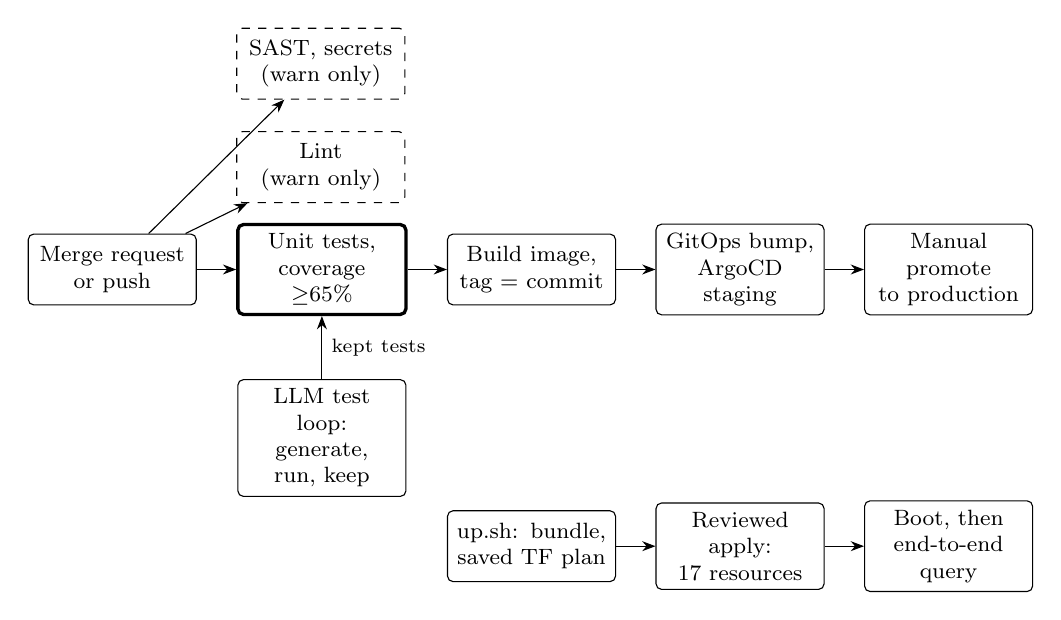
\begin{tikzpicture}[font=\linespread{1}\footnotesize, >=Stealth, node distance=4mm and 5mm,
  st/.style={draw, rounded corners=2pt, align=center, minimum height=9mm, text width=19mm, fill=white},
  gate/.style={st, very thick},
  warn/.style={st, dashed}]
\node[st] (mr) {Merge request\\or push};
\node[warn, right=of mr, yshift=13mm] (lint) {Lint\\(warn only)};
\node[gate, right=of mr] (ut) {Unit tests,\\coverage $\ge$65\%};
\node[warn, above=4mm of lint] (sast) {SAST, secrets\\(warn only)};
\node[st, below=8mm of ut] (gen) {LLM test loop:\\generate, run, keep};
\node[st, right=of ut] (build) {Build image,\\tag = commit};
\node[st, right=of build] (stg) {GitOps bump,\\ArgoCD staging};
\node[st, right=of stg] (prod) {Manual promote\\to production};
\node[st, below=26mm of build] (tf) {up.sh: bundle,\\saved TF plan};
\node[st, right=of tf] (apply) {Reviewed apply:\\17 resources};
\node[st, right=of apply] (smoke) {Boot, then\\end-to-end query};
\draw[->] (mr) -- (lint); \draw[->] (mr) -- (ut); \draw[->] (mr) -- (sast);
\draw[->] (gen) -- node[right, font=\scriptsize]{kept tests} (ut);
\draw[->] (ut) -- (build); \draw[->] (build) -- (stg); \draw[->] (stg) -- (prod);
\draw[->] (tf) -- (apply); \draw[->] (apply) -- (smoke);
\end{tikzpicture}
\caption{Delivery workflow. Solid thick box: blocking gate; dashed boxes: warn-only checks. The lower row is the one-command Terraform deployment used for the evaluated system.}
\label{fig:cicd}
\end{figure}

\section{Experimental Setup}

\textbf{Data.} The corpus is the email of EZO Books, an accounting-software company of 53 users, collected with the client's consent. After filtering and extraction the graph holds 11,584 threads, 27,063 content nodes, 13,562 Person and 3,609 Topic nodes and 85,392 typed relationships; 4,631 tasks have an assignee and 4,658 decisions have a stated reason.

\textbf{Golden evaluation set.} Both test sets were built once and frozen as versioned files before any system was run, so every configuration is scored against the same questions and labels. Test A has 55 relationship questions generated from three Cypher templates with a fixed seed: tasks of a person (15), why a decision was made (20) and what a person decided about a topic (20). Its ground truth is the Cypher result for the pattern, 268 nodes in total. Ambiguous names are removed and person answers must span at least two threads. Test B has 60 single-email lookups: an LLM wrote one question from the raw text of each sampled thread, and the label is that thread. Test B is a control, where the graph should not help.

\textbf{Baselines.} \emph{Raw RAG} indexes raw email threads, and \emph{node RAG} indexes the extracted node texts, both built with LangChain's vector-store interface \cite{langchain2026vectorstores} over FAISS \cite{johnson2017faiss} and the same embedding model as Lore. Node RAG sees exactly the text the graph holds, so it isolates the contribution of graph structure.

\textbf{Metrics.} \emph{Node recall@10}, $|\mathcal{G}_q\cap R_{10}(q)|/\min(|\mathcal{G}_q|,10)$, measures how much of the answer is found without penalising questions with many answers. \emph{Thread recall@10} applies the same formula to source threads and is the only fair metric for raw RAG. \emph{Hit@$k$} records whether the source thread is in the top $k$, and \emph{MRR@10} rewards ranking it first. \emph{Median latency} reflects interactive use. Each configuration was run once against the frozen golden set. Every mean is reported with its bootstrap standard error, the standard deviation of the mean over 5,000 resamples of the questions, and differences between systems are paired over questions and reported with a 95\% bootstrap interval \cite{efron1993bootstrap}. These quantify uncertainty from the choice of questions; variation between repeated runs of the LLM analysis is not included.

\textbf{Environment.} Python 3.12, FastAPI, Neo4j 5.26 Community, PostgreSQL 16 with pgvector, FlashRank 0.2, LangChain with FAISS-CPU, and Claude 3.5 Sonnet v2 through the Bedrock APAC inference profile. All services ran in Docker on a single developer workstation, with the engine started once per configuration on its own port and each harness calling it over HTTP exactly as the user interface does. The unit tests use pytest with pytest-cov; the test generator calls \texttt{nemotron-3-super-120b} through the NVIDIA API at temperature 0.2 with up to three attempts per module. The ablation switches the reranker off with \texttt{RERANK\_PROVIDER=none} and forces the keyword analysis with \texttt{ANALYSIS\_TIMEOUT\_MS=1}. The BM25 library was not installed in the evaluation environment, so $h=\hat{g}$ in every run reported here. Table~\ref{tab:params} lists all settings.

\begin{table}[t]
\centering
\caption{Parameters used in all experiments}
\label{tab:params}
\footnotesize
\begin{tabular}{@{}ll@{}}
\toprule
Setting & Value \\
\midrule
Embedding model & \texttt{nvidia/nemotron-3-embed-1b}, 2048 dimensions \\
Analysis and answer LLM & Claude 3.5 Sonnet v2 (Bedrock), analysis deadline 4,000 ms \\
Vector seeds / beam width / depth & 30 / 30 / 3 \\
Hop penalties $h_1,h_2,h_3$; $\gamma$ & 1.0, 0.8, 0.6; 0.1 \\
$\alpha, \beta$ (hybrid); $w_1, w_2$ (final) & 0.6, 0.4 (BM25 inactive); 0.7, 0.3 \\
Cross-encoder & FlashRank \texttt{ms-marco-MiniLM-L-12-v2} \\
Context budget; $k$ & 8,000 tokens; 10 \\
Question seeds & 7 (Test A), 42 (Test B) \\
Bootstrap & 5,000 resamples, seed 0 \\
Runs per configuration & 1 (uncertainty: bootstrap standard error over questions) \\
\bottomrule
\end{tabular}
\end{table}

\section{Results and Analysis}

\subsection{RQ1: graph retrieval against vector RAG}
Table~\ref{tab:testa} reports Test A. Lore's node recall@10 is $0.40 \pm 0.06$ against $0.14 \pm 0.04$ for node RAG, a paired difference of +0.26 with a 95\% interval of [+0.13, +0.40]. Fig.~\ref{fig:families} breaks this down by question family. The largest gain is on ``person on topic'' (0.38 against 0.01), where the answer is the intersection of a person and a topic: the graph reaches it through DECIDED and REGARDING edges, while vector search cannot match a name that does not appear in the decision text. ``Tasks of a person'' improves from 0.03 to 0.10, which is significant but low in absolute terms; we return to it in Section VII. ``Why decided'' rises from 0.35 to 0.65, but its interval [$-0.05$, +0.60] touches zero, so we treat it as a trend. On thread recall Lore leads overall (0.50 against 0.35 for node RAG and 0.33 for raw RAG), while raw RAG finds the thread of a decision question slightly more often (0.82 against 0.77), because the decision wording appears in the email itself. The ``why decided'' family shows the difference between the two metrics clearly: every system finds the right thread, but only Lore reliably returns the specific Fact node that states the reason, because it follows the BECAUSE edge from the decision instead of returning the most similar text.

The cause of the gain can be checked directly in the data. Of the 144 correct task descriptions in ``tasks of a person'', only 6 (4\%) contain any token of the person's name, and of the 100 correct decisions in ``person on topic'' only 1 does. An embedding of ``What tasks were assigned to $X$?'' therefore has nothing in the answer text to match, which explains why node RAG scores near zero on both families while it performs reasonably on ``why decided'', whose question repeats the decision text.

\begin{table}[t]
\centering
\caption{Test A (55 relationship questions): recall@10 as mean $\pm$ bootstrap standard error over questions, and median latency. Best value per column in bold.}
\label{tab:testa}
\scriptsize
\setlength{\tabcolsep}{3.5pt}
\begin{tabular}{@{}lccccc@{}}
\toprule
System and metric & Tasks of person & Why decided & Person on topic & All & Latency \\
\midrule
Raw RAG, thread recall & $0.06 \pm 0.03$ & $\mathbf{0.82} \pm 0.08$ & $0.04 \pm 0.02$ & $0.33 \pm 0.06$ & 0.37 s \\
Node RAG, thread recall & $0.16 \pm 0.03$ & $\mathbf{0.82} \pm 0.08$ & $0.02 \pm 0.01$ & $0.35 \pm 0.06$ & \textbf{0.35 s} \\
Lore, thread recall & $\mathbf{0.17} \pm 0.04$ & $0.77 \pm 0.09$ & $\mathbf{0.49} \pm 0.09$ & $\mathbf{0.50} \pm 0.06$ & 8.0 s \\
\midrule
Node RAG, node recall & $0.03 \pm 0.01$ & $0.35 \pm 0.11$ & $0.01 \pm 0.01$ & $0.14 \pm 0.04$ & \textbf{0.35 s} \\
Lore, node recall & $\mathbf{0.10} \pm 0.03$ & $\mathbf{0.65} \pm 0.11$ & $\mathbf{0.38} \pm 0.09$ & $\mathbf{0.40} \pm 0.06$ & 8.0 s \\
Lore $-$ node RAG & +0.08 & +0.30 & +0.37 & +0.26 & \\
\quad paired 95\% CI & [+0.02, +0.15] & [$-$0.05, +0.60] & [+0.19, +0.56] & [+0.13, +0.40] & \\
\bottomrule
\end{tabular}
\end{table}

\begin{figure}[t]
\centering
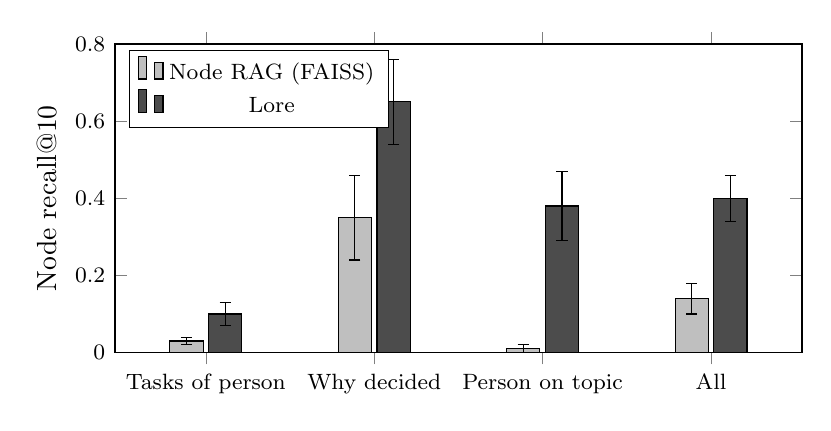
\begin{tikzpicture}
\begin{axis}[ybar, width=0.85\textwidth, height=5.5cm, bar width=12pt, ymin=0, ymax=0.8,
  ylabel={Node recall@10}, symbolic x coords={Tasks of person, Why decided, Person on topic, All},
  xtick=data, enlarge x limits=0.18, legend style={at={(0.02,0.98)}, anchor=north west, font=\footnotesize},
  tick label style={font=\footnotesize}]
\addplot[fill=black!25, error bars/.cd, y dir=both, y explicit] coordinates {(Tasks of person,0.03) +- (0,0.01) (Why decided,0.35) +- (0,0.11) (Person on topic,0.01) +- (0,0.01) (All,0.14) +- (0,0.04)};
\addplot[fill=black!70, error bars/.cd, y dir=both, y explicit] coordinates {(Tasks of person,0.10) +- (0,0.03) (Why decided,0.65) +- (0,0.11) (Person on topic,0.38) +- (0,0.09) (All,0.40) +- (0,0.06)};
\legend{Node RAG (FAISS), Lore}
\end{axis}
\end{tikzpicture}
\caption{Node recall@10 on Test A by question family; error bars show one bootstrap standard error. The gap is largest where the answer is linked to the question only by edges.}
\label{fig:families}
\end{figure}

Table~\ref{tab:testb} reports Test B, the control. Vector RAG over raw threads wins clearly: hit@10 $0.75 \pm 0.06$ against $0.40 \pm 0.06$, and MRR@10 0.56 against 0.33. This matches the prediction of Han et al.\ \cite{han2025ragvsgraphrag}: when question and answer share wording, similarity search is already the right tool. Lore is also about ten times slower on lookups (5.9 s against 0.5 s) and twenty times slower on relationship questions, because each request makes an analysis call, several Cypher queries and a cross-encoder pass before the answer call.

\begin{table}[t]
\centering
\caption{Test B (60 single-email lookups), mean $\pm$ bootstrap standard error over questions. Best value per column in bold.}
\label{tab:testb}
\footnotesize
\begin{tabular}{@{}lcccc@{}}
\toprule
System & Hit@1 & Hit@10 & MRR@10 & Median latency \\
\midrule
Vector RAG over raw threads & $\mathbf{0.47} \pm 0.07$ & $\mathbf{0.75} \pm 0.06$ & $\mathbf{0.56} \pm 0.06$ & \textbf{0.5 s} \\
Lore & $0.28 \pm 0.06$ & $0.40 \pm 0.06$ & $0.33 \pm 0.06$ & 5.9 s \\
\bottomrule
\end{tabular}
\end{table}

\subsection{RQ2: ablation of query analysis and reranking}
Table~\ref{tab:ablation} switches the two query-time components on and off, with the graph, questions and all other settings fixed; the keyword, reranker-off cell is an earlier run in which the reranker was not installed and the analysis deadline of 800 ms made it fall back to keywords on almost every query. Two effects stand out. First, LLM analysis is a trade-off: with the reranker on it raises ``person on topic'' by +0.32 [+0.14, +0.50] and all of Test A by +0.12 [+0.02, +0.23], but lowers Test B hit@10 by $-0.23$ [$-0.35$, $-0.12$]. Second, the reranker matters only after LLM analysis: it adds +0.27 [+0.17, +0.38] on lookups and +0.09 on ``tasks of a person'', while with keyword analysis it changes nothing on lookups, and 52 of 60 questions keep the same rank. Fig.~\ref{fig:ablation} makes the interaction visible. Our reading is that LLM analysis widens the candidate set towards people and topics, which helps relational questions and pushes the source email of a lookup below rank 10, and the cross-encoder then pulls it back up. This explanation has not yet been tested directly. The components also change cost: median Test A latency is 8.0 s with both on, 7.0 s without the reranker and 6.4 s with keyword analysis, and on Test B the reranker-on, LLM configuration also has the best hit@1 among LLM-analysis cells (0.28 against 0.05 without the reranker). No single configuration wins both tests, which is the strongest argument in this study for routing questions by type rather than tuning one pipeline for all of them.

Table~\ref{tab:failures} classifies the remaining errors using the failure points of Barnett et al.\ \cite{barnett2024failure}. Most of them are ranking failures: the right node was reachable but did not reach the top ten. Only recency questions over code fail because the content itself is missing, since the code index has no usable commit dates.

\begin{table}[t]
\centering
\caption{Error analysis of the shipped configuration}
\label{tab:failures}
\footnotesize
\begin{tabularx}{\textwidth}{@{}>{\raggedright\arraybackslash}p{3.1cm}Y>{\raggedright\arraybackslash}p{3.2cm}Y@{}}
\toprule
Failure & Evidence & Failure point \cite{barnett2024failure} & Likely cause \\
\midrule
Single-email lookups & hit@10 0.40 against 0.75 & Missed top-ranked documents & LLM analysis widens candidates ($-0.23$ in ablation) \\
Tasks of a person & node recall 0.10; up to 18 answers for 10 slots & Not in context & Person hubs have hundreds of edges; beam keeps 30 (hypothesis) \\
Why decided (node level) & 0.65, interval touches zero against baseline & Missed top-ranked documents & Small family (20 questions) \\
Recency of code changes & ``most recent change'' unanswerable & Missing content & No usable commit dates in the code index \\
\bottomrule
\end{tabularx}
\end{table}

\begin{table}[t]
\centering
\caption{2$\times$2 ablation, mean $\pm$ bootstrap standard error over questions. Test A: node recall@10; Test B: hit@10 and MRR@10.}
\label{tab:ablation}
\scriptsize
\setlength{\tabcolsep}{3pt}
\begin{tabular}{@{}lcccccc@{}}
\toprule
Reranker, analysis & A: all & A: tasks & A: why & A: topic & B: hit@10 & B: MRR \\
\midrule
On, LLM (shipped) & $\mathbf{0.40} \pm 0.06$ & $0.10 \pm 0.03$ & $0.65 \pm 0.11$ & $0.38 \pm 0.09$ & $0.40 \pm 0.06$ & $0.33 \pm 0.06$ \\
Off, LLM & $\mathbf{0.40} \pm 0.07$ & $0.01 \pm 0.01$ & $\mathbf{0.70} \pm 0.10$ & $\mathbf{0.39} \pm 0.10$ & $0.13 \pm 0.04$ & $0.07 \pm 0.03$ \\
On, keywords & $0.28 \pm 0.06$ & $0.09 \pm 0.02$ & $0.65 \pm 0.11$ & $0.06 \pm 0.05$ & $\mathbf{0.63} \pm 0.06$ & $0.51 \pm 0.06$ \\
Off, keywords & $0.31 \pm 0.06$ & $\mathbf{0.20} \pm 0.04$ & $\mathbf{0.70} \pm 0.10$ & $0.01 \pm 0.01$ & $\mathbf{0.63} \pm 0.06$ & $\mathbf{0.52} \pm 0.06$ \\
\bottomrule
\end{tabular}
\end{table}

\begin{figure}[t]
\centering
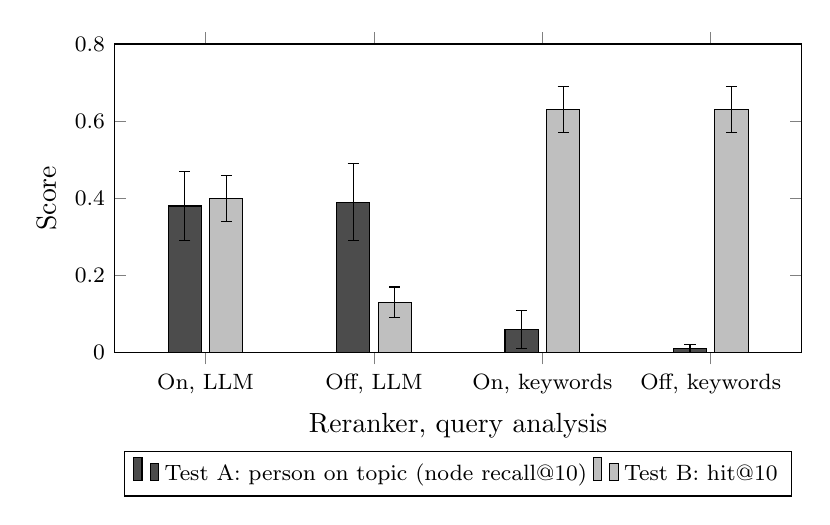
\begin{tikzpicture}
\begin{axis}[ybar, width=0.85\textwidth, height=5.5cm, bar width=12pt, ymin=0, ymax=0.8,
  ylabel={Score}, symbolic x coords={{On, LLM}, {Off, LLM}, {On, keywords}, {Off, keywords}},
  xtick=data, xlabel={Reranker, query analysis}, enlarge x limits=0.18,
  legend style={at={(0.5,-0.32)}, anchor=north, legend columns=2, font=\footnotesize}, ybar=3pt,
  tick label style={font=\footnotesize}]
\addplot[fill=black!70, error bars/.cd, y dir=both, y explicit] coordinates {({On, LLM},0.38) +- (0,0.09) ({Off, LLM},0.39) +- (0,0.10) ({On, keywords},0.06) +- (0,0.05) ({Off, keywords},0.01) +- (0,0.01)};
\addplot[fill=black!25, error bars/.cd, y dir=both, y explicit] coordinates {({On, LLM},0.40) +- (0,0.06) ({Off, LLM},0.13) +- (0,0.04) ({On, keywords},0.63) +- (0,0.06) ({Off, keywords},0.63) +- (0,0.06)};
\legend{Test A: person on topic (node recall@10), Test B: hit@10}
\end{axis}
\end{tikzpicture}
\caption{Ablation, with one bootstrap standard error per bar. LLM analysis drives relational recall (dark bars) and lowers lookup accuracy (light bars); the reranker recovers lookups only when LLM analysis is on.}
\label{fig:ablation}
\end{figure}

\subsection{Automation pipeline outcomes}
Table~\ref{tab:testgen} reports the LLM test generator on four modules. Three modules reached 100\% line coverage after one or two attempts and their tests were kept; the fourth produced tests that did not raise coverage after three attempts and was rejected, which is the intended behaviour of the filter. The suite grew from 266 to 307 tests and total coverage from 66\% to 68\%, above the 65\% gate; a fresh run gives 306 passed and 1 skipped. The course-branch pipeline completed lint, tests, scans and build successfully. The Terraform stack went from apply to a working HTTPS site in about five minutes; an end-to-end query through the deployed system returned an answer with ten cited sources in 11 to 17 seconds, and requests without the password received HTTP 401. Memory peaked at 1.2 GiB during a live query, so the instance was cut from a t3.xlarge (US\$4.5 per day) to a t3.large (\$2.4 per day), and the stack can be destroyed with one command, which made it practical to run the demonstration only when needed and to rebuild it from scratch after the instance had been stopped.

\begin{table}[t]
\centering
\caption{LLM test generation (generate, run, keep only if passing and coverage rises)}
\label{tab:testgen}
\footnotesize
\begin{tabular}{@{}lcccc@{}}
\toprule
Module & Coverage before & Coverage after & Attempts & Kept \\
\midrule
\texttt{domain/sources.py} & 40.6\% & \textbf{100\%} & 2 & yes \\
\texttt{domain/retrieval/person.py} & 40.8\% & \textbf{100\%} & 2 & yes \\
\texttt{domain/scoring.py} & 61.9\% & \textbf{100\%} & 1 & yes \\
\texttt{domain/context.py} & 39.3\% & 39.3\% & 3 & no \\
\bottomrule
\end{tabular}
\end{table}

\section{Discussion}

The results answer a practical question for any organisation that wants an assistant over its mail: a typed graph is worth building when people ask about who did what and why, and it is a poor choice for finding a half-remembered email. The two cases call for different tools, so the most useful next component is a router that sends lookup-style questions to plain retrieval and relational questions to the graph path. The ablation also gives an engineering lesson. The earlier run, in which an optional dependency was missing and a timeout was too short, scored 0.01 on ``person on topic'' without any test failing; the 2$\times$2 design showed that the timeout, not the missing reranker, caused the drop. Pinning dependencies in the image and logging every fallback were therefore as important as the retrieval algorithm itself.

``Tasks of a person'' stays low (0.10) because a person with many assignments is a hub with hundreds of edges, while the beam keeps 30 candidates and the answer list has 10 slots for up to 18 correct tasks. This is a hypothesis from logs, not a measured cause; personalised PageRank \cite{gutierrez2024hipporag} spreads over all edges of a hub and is the obvious experiment.

The study has clear limitations. It covers one organisation and 15 to 20 questions per family, so several intervals are wide. Each configuration was run once, so our error bars reflect the choice of questions, not the run-to-run variation of the LLM analysis, which is not yet measured. Ground truth comes from the same LLM-extracted graph, so an extraction error counts as truth and the templates favour the structure the graph encodes; Test B, whose labels come from raw email, partly offsets this. We measure retrieval, not the quality of the written answer, and BM25 was inactive in every run.

\emph{Ethics.} The data is a client's private email, used with consent. No email text, extracted graph or per-question output is in the code repository: questions are regenerated from the graph, every node carries access scopes that the engine enforces inside each query, phone numbers are redacted before synthesis, and the deployed demo sits behind a password and stores its secrets encrypted.

\section{Conclusion and Future Work}

For RQ1, retrieval over an ontology-typed email graph raises node recall@10 on relationship questions from 0.14 to 0.40 (+0.26, 95\% CI [+0.13, +0.40]) but loses on single-email lookups (hit@10 0.40 against 0.75) and is about twenty times slower. For RQ2, LLM query analysis causes both the largest gain (+0.32 on person-and-topic questions) and the lookup loss ($-0.23$), and the cross-encoder recovers +0.27 on lookups only when that analysis is on. The surrounding workflow, a coverage-gated CI stage fed by a filtered LLM test generator and a one-command infrastructure-as-code deployment, made the system testable and shippable by a small team: three modules reached full line coverage, a fourth was correctly rejected, and the whole system could be recreated on AWS in about five minutes. For an organisation, the practical message is to treat relational questions and lookups as different products, and to measure each component before trusting it. Three directions follow. First, add a question router and measure whether it keeps the relational gain while restoring lookup accuracy. Second, test personalised PageRank on person hubs. Third, add an answer-quality score with human labels on a sample, and rerun every configuration several times to report its variance.

\section*{Code Availability}
Code, evaluation scripts, CI pipeline, Terraform and this paper (private; faculty have access):\\
\url{https://github.com/ninadw25/AI_devops_loremind}

\section*{AI-Use Declaration}
% TODO(team): keep this accurate. Add any other tools you used (e.g. ChatGPT, Grammarly) and remove anything you did not use.
LLMs are components of the system described here (triple extraction, query analysis, answer synthesis, question and test generation). The team used Claude (Anthropic), through Claude Code, to write code and evaluation scripts, draw figures, and draft and edit text. All results come from running the code; the authors rewrote the text and checked every number and reference.

\section*{Contribution Statement}
% TODO(team): one line per member.
\noindent Name1: [contribution].\\
Name2: [contribution].\\
Name3: [contribution].

\bibliographystyle{IEEEtran}
\bibliography{references}

\end{document}
